\chapter{怎样寻找优质的教程}
\label{cha:how-to-find-tutorials}

\begin{intro}
  在软件篇开篇时我们就强调过,《你缺失的那门计算机课》不会是任何一款具体软件的教程。这是由这份教程的编写初衷决定的——每个人所需要掌握的软件都不一样,要学习的具体方面更是千差万别,本书无法,也不可能成为一个人人都能取用的大杂烩。相反地,我们在这里向大家介绍「怎样寻找优质的教程」。
\end{intro}

一份好的软件教程能帮助我们更快、更熟练地使用软件。今天,互联网上的内容多如牛毛,但像《你缺计课》这样用心编写的优质教程却少之又少。寻找优质软件教程,如同沙里淘金,这一章将向你介绍一些可能更容易找到优质教程的方法。

\section{利用好软件的官方文档}

在许多时候,软件的开发商会为自己的产品撰写文档。这些文档往往可以免费在互联网上获取到,而且相当权威和准确。将官方文档作为学习参考,不失一种不错的选择。

例如,如果你想学习 Excel 软件中「函数」部分的使用,那么可以查阅微软官方的 Excel 文档,例如位于 \url{https://support.microsoft.com/zh-cn/office/excel-函数-按类别列出-5f91f4e9-7b42-46d2-9bd1-63f26a86c0eb} 的这一份。

\begin{figure}[htb!]
  \centering
  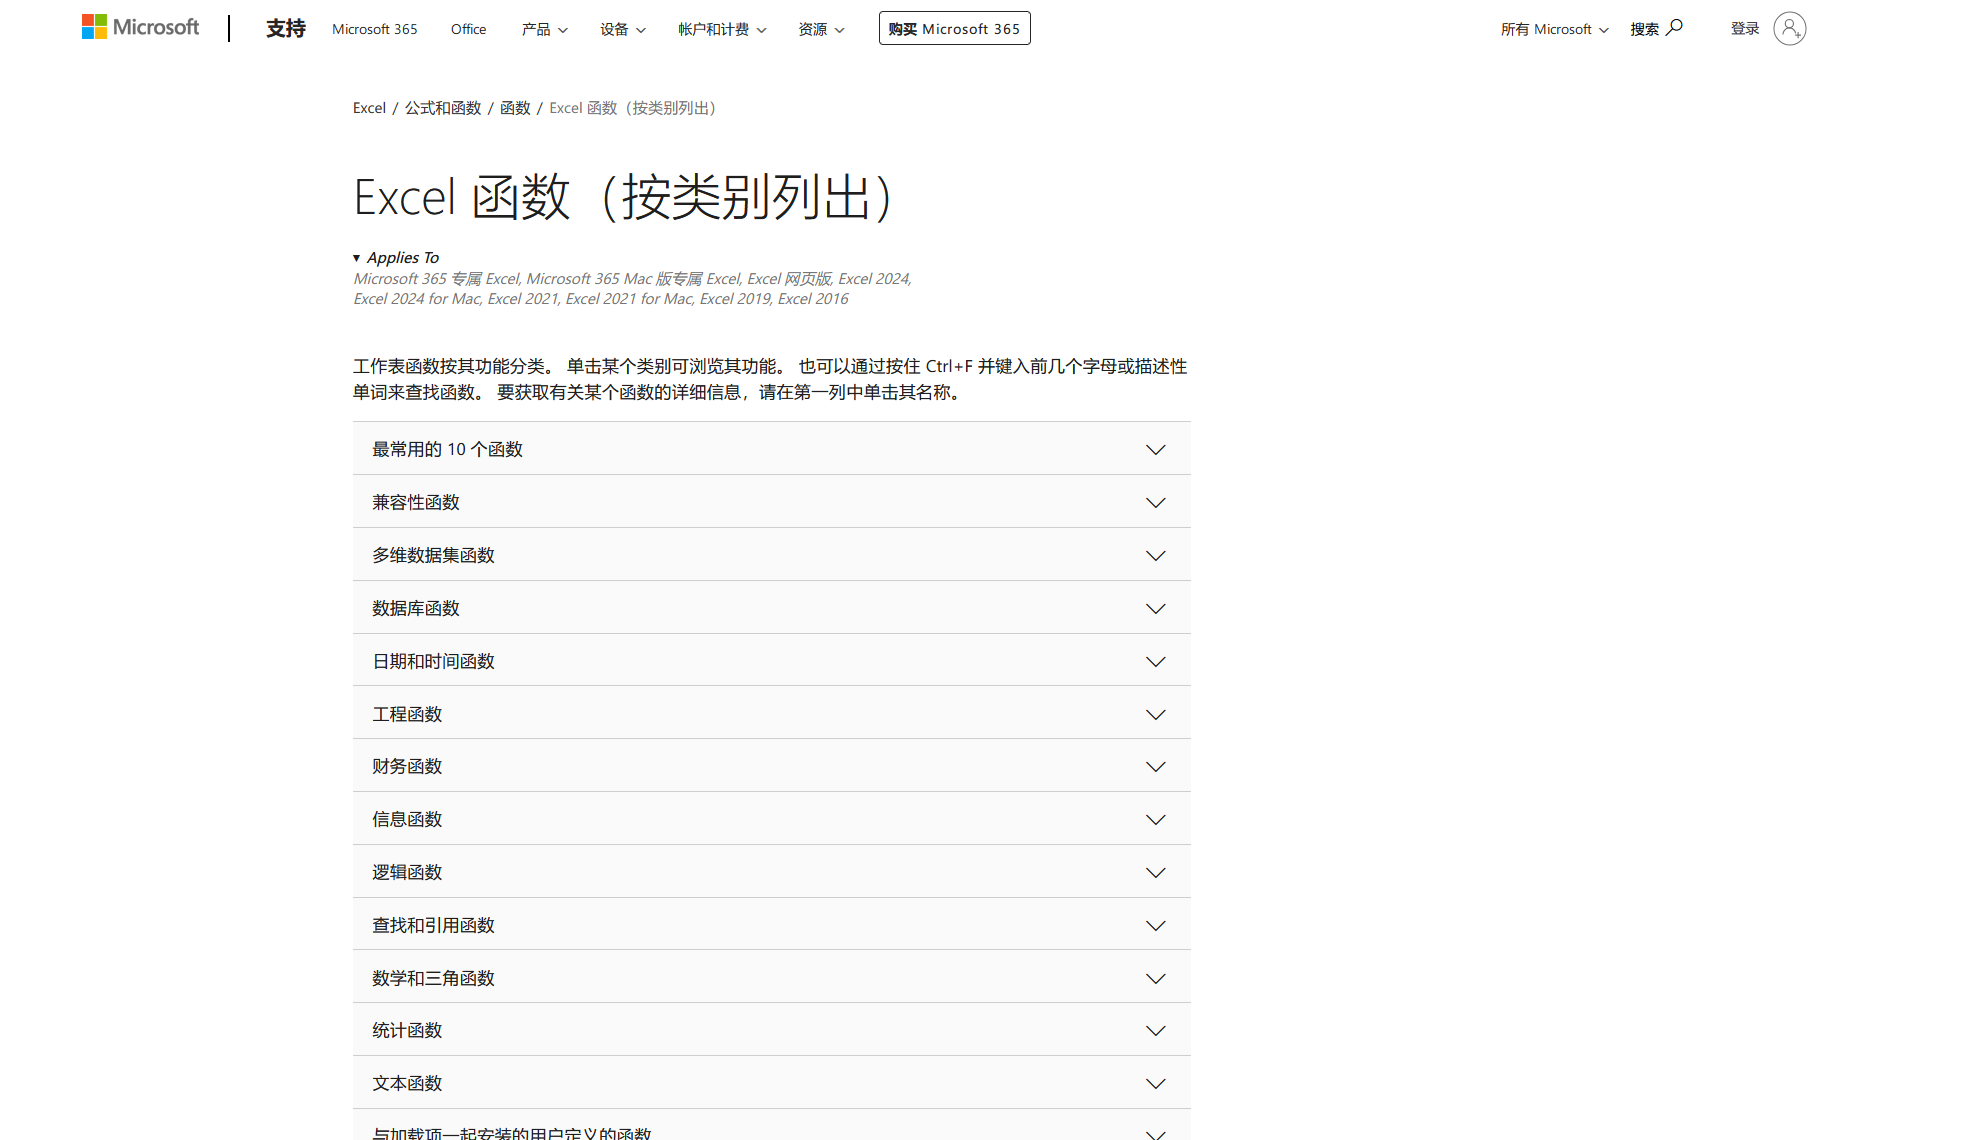
\includegraphics[width=.9\textwidth]{assets/software/MS_document_for_Excel.png}
  \caption{微软官方的 Excel 函数文档}
  \label{fig:MS_document_for_Excel}
\end{figure}

这份官方文档不仅对每个常用的 Excel 函数都有介绍,并且还附上了示例和教学视频,因而比较容易学习。下面是 \MissingVerb{SUM} 函数的介绍、示例和视频:

\begin{figure}[htb!]
  \centering
  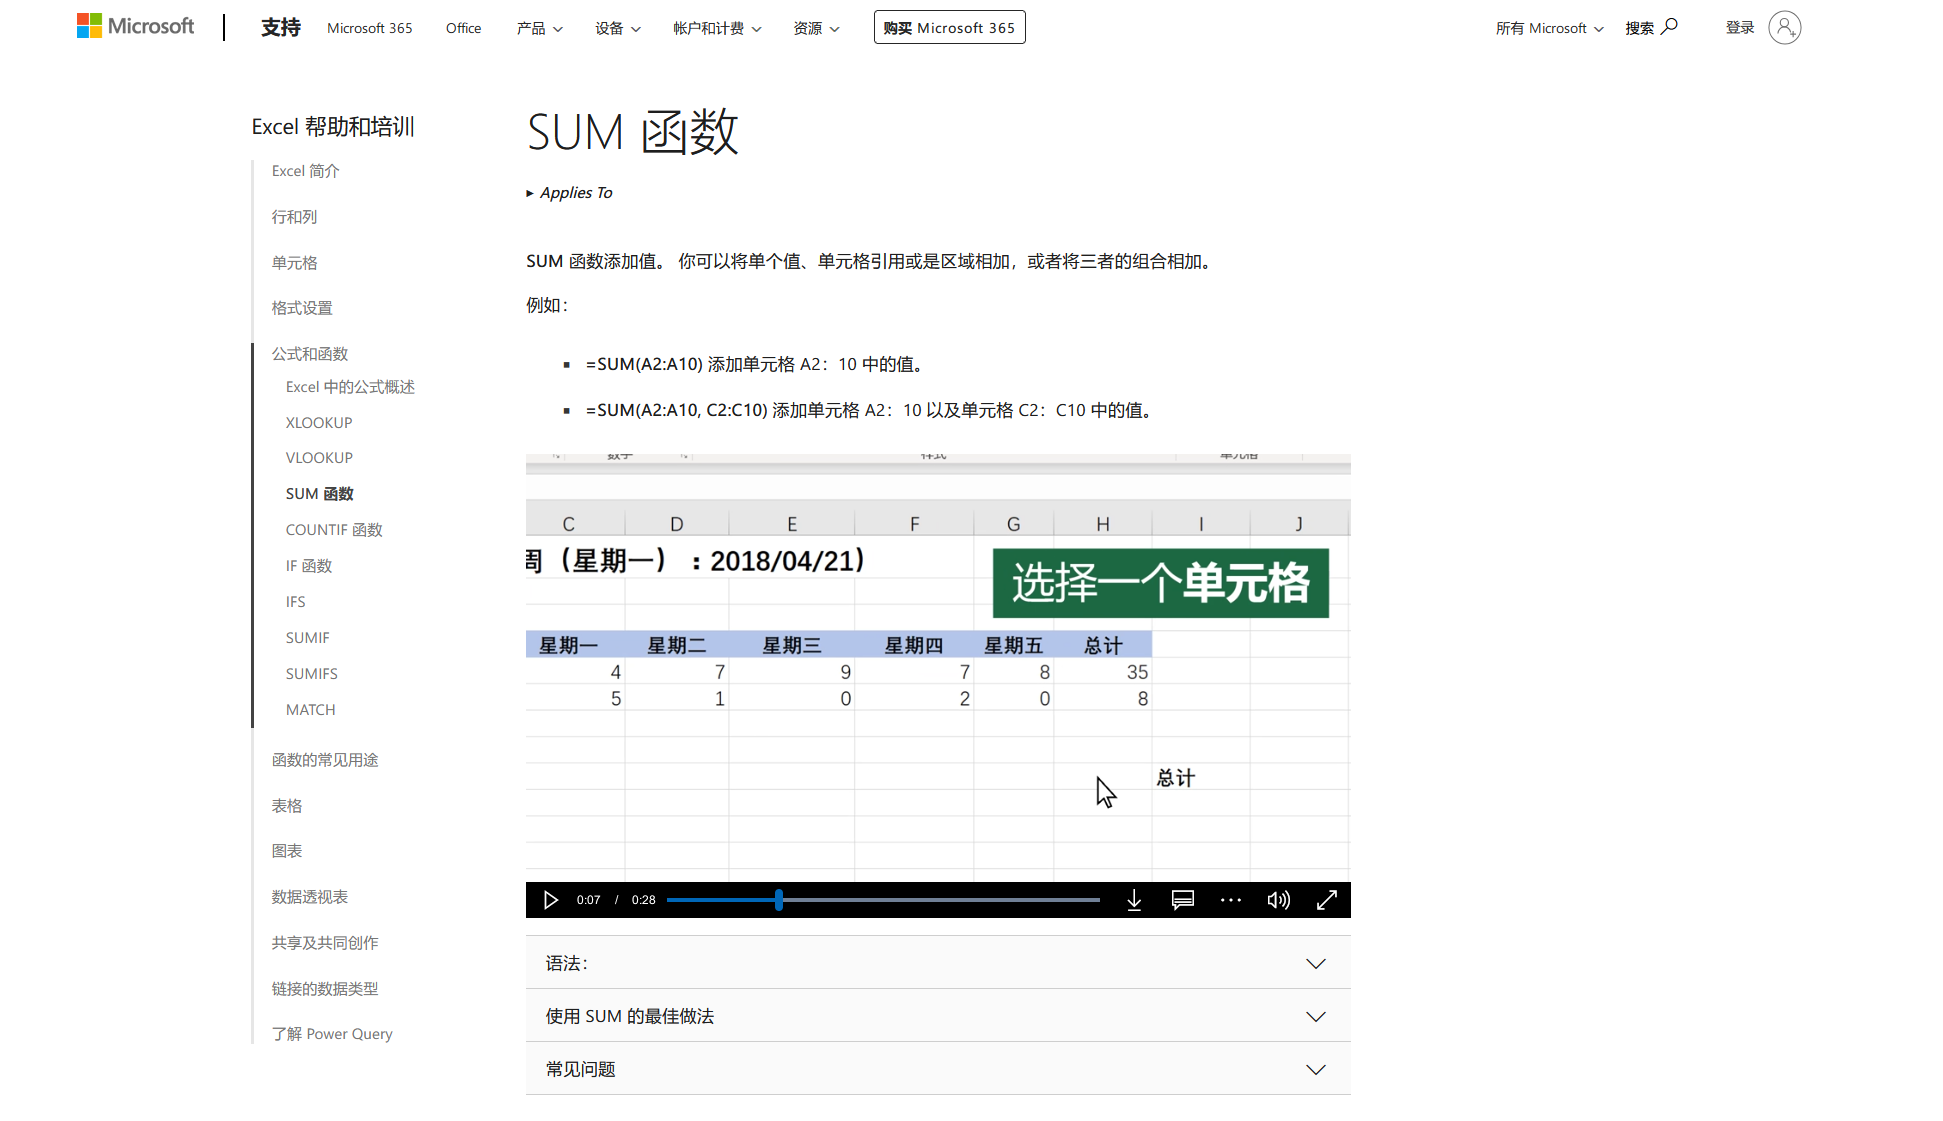
\includegraphics[width=.85\textwidth]{assets/software/MS_document_for_Excel_2.png}
  \caption{\MissingTT{SUM} 详解}
  \label{fig:MS_document_for_Excel_1}
\end{figure}

又比如说,你想了解 Photoshop 的使用,那么 Adobe 官方也有制作一套详细的文档,位于 \url{https://helpx.adobe.com/cn/photoshop/user-guide.html}。

\begin{figure}[htb!]
  \centering
  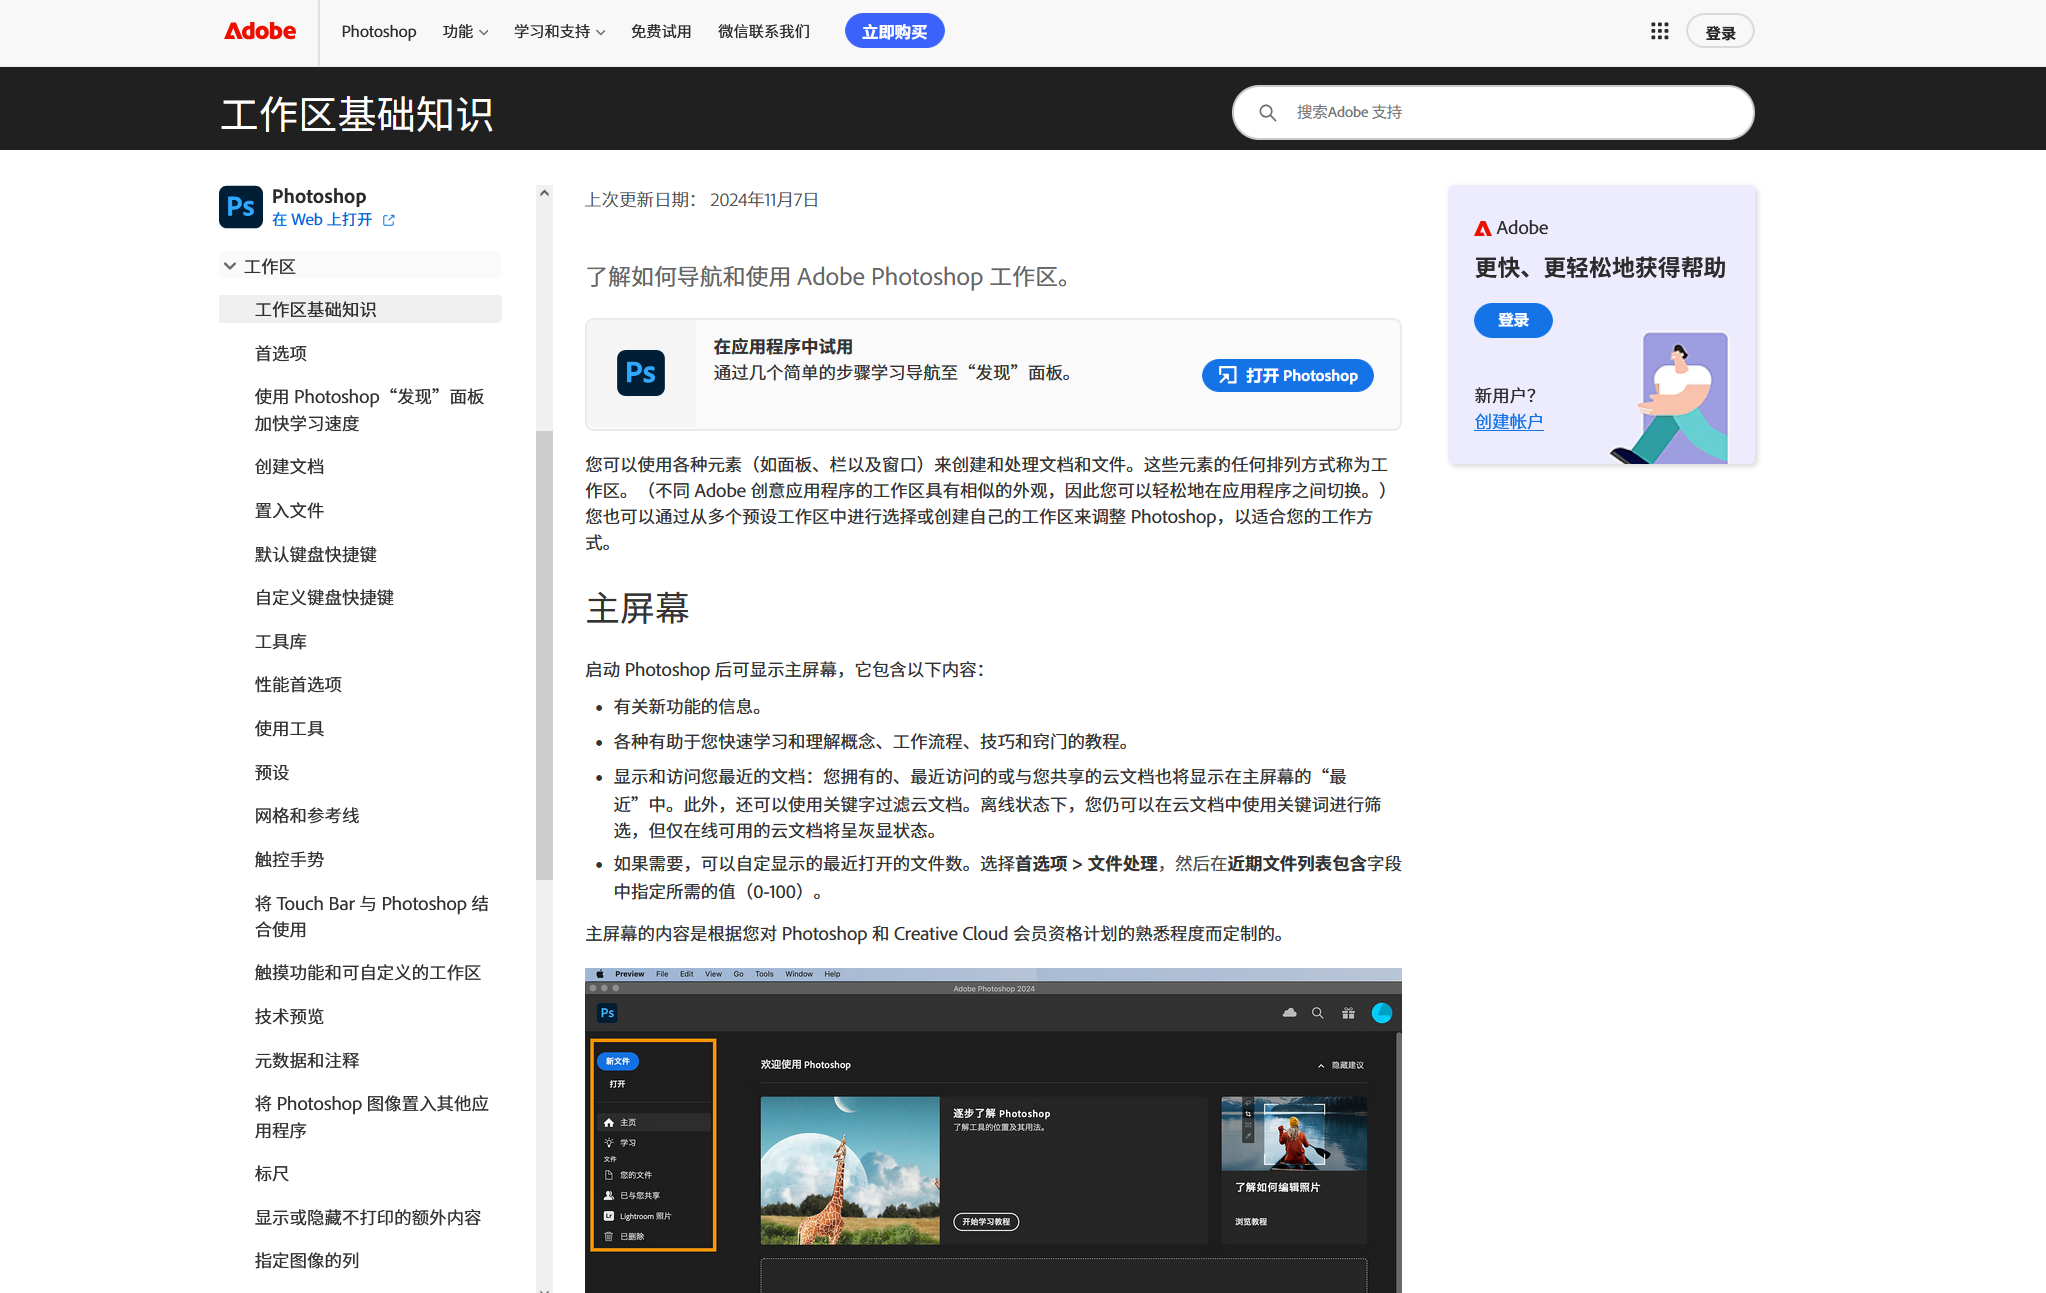
\includegraphics[width=.8\textwidth]{assets/software/Adobe_document_for_PS.png}
  \caption{Adobe 官方推出的 Photoshop 教程}
  \label{fig:Adobe_document_for_PS}
\end{figure}

一般来说,我们可以通过访问软件的官方网站(不知道怎么找?请参看\chapref{cha:software-installation}),并在官方网站寻找名为「帮助」或「支持」的栏目来查找官方文档/官方教程。此外,你也可以直接在网上搜索「\texttt{<软件名>\ 官方文档}」「\texttt{<软件名>\ 帮助\ 支持}」等来尝试直接寻找相关的官方文档。

还有一些软件,可以在安装时将文档一同安装到你电脑上,或可以在安装软件之后加装本地文档。这样,我们就不用总是到网上寻找资料,而是任何时候都能在本地阅读文档、学习软件了。

例如,如果你想学习使用「Mathematica」这款数学计算软件\CJKsout*{(高级计算器)},可以在安装它的时候选装本地文档。在启动 Mathematica 后,随时按下 \keys{F1},就能前往安装好的本地文档。

\begin{figure}[htb!]
  \centering
  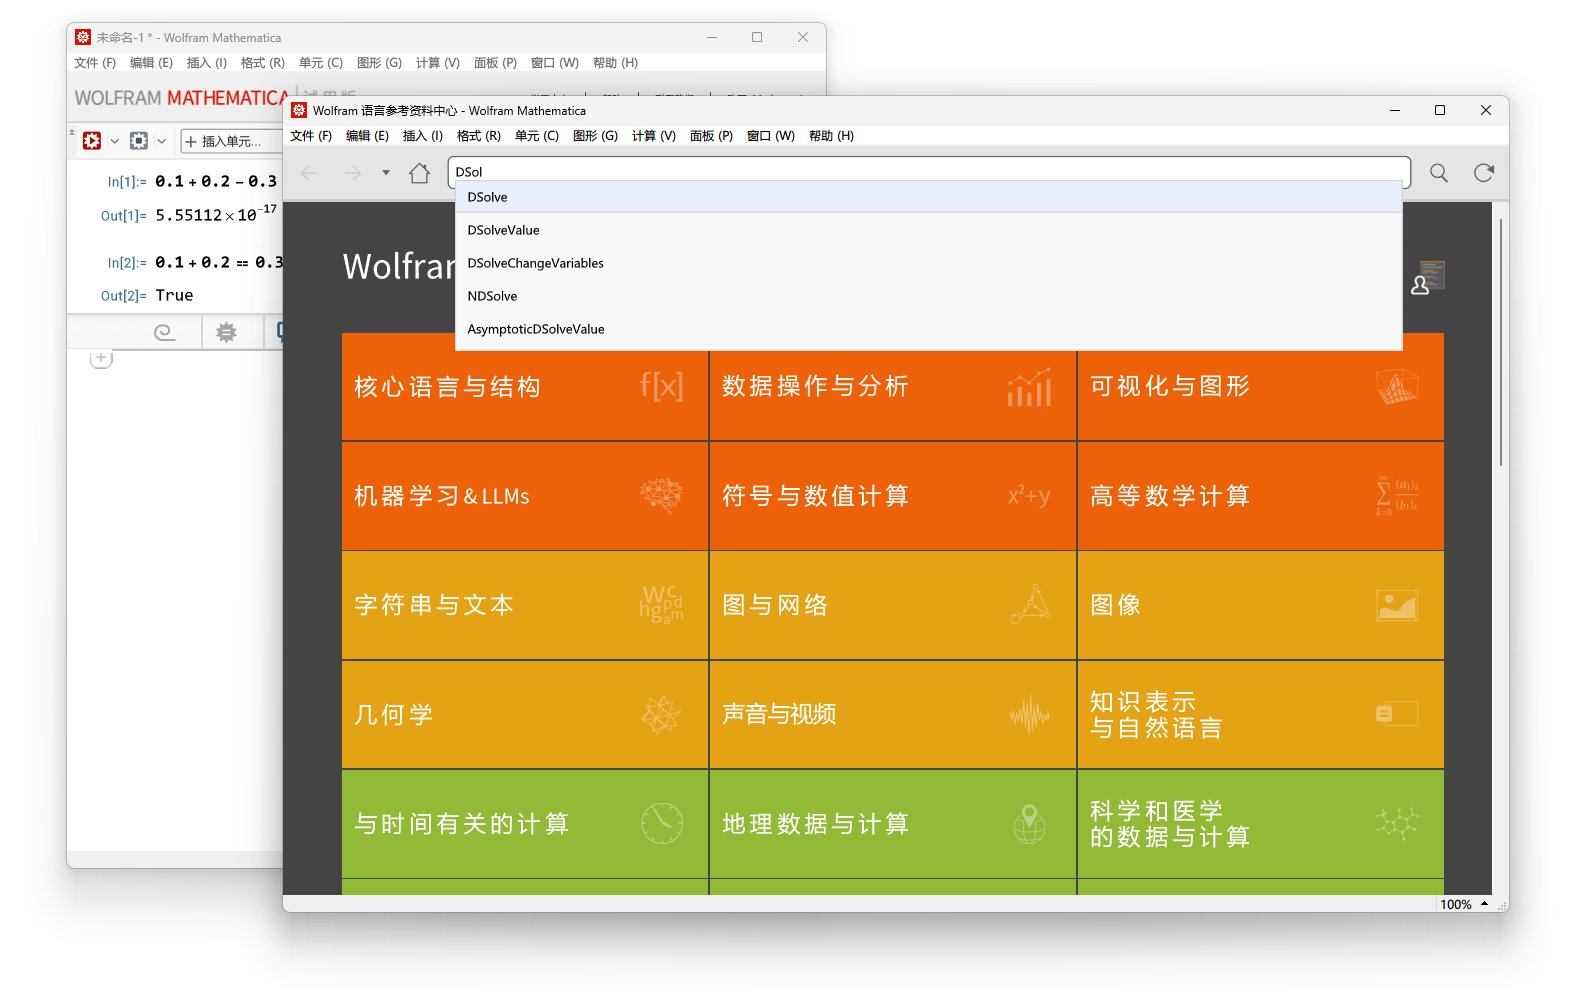
\includegraphics[width=.8\textwidth]{assets/software/MMA_document.png}
  \caption{Mathematica 的本地文档}
  \label{fig:MMA_document}
\end{figure}

值得一提的是,Mathematica 的文档是全中文、可交互的,可以说是最优秀的本地中文文档之一。所以你可以用中文作为关键词搜索文档内容,找到自己想要的指令。你也可以在文档页面中自己试试计算它给出的示例,甚至改写示例、新增算例来即时检验你的学习成果。

\begin{figure}[htb!]
  \centering
  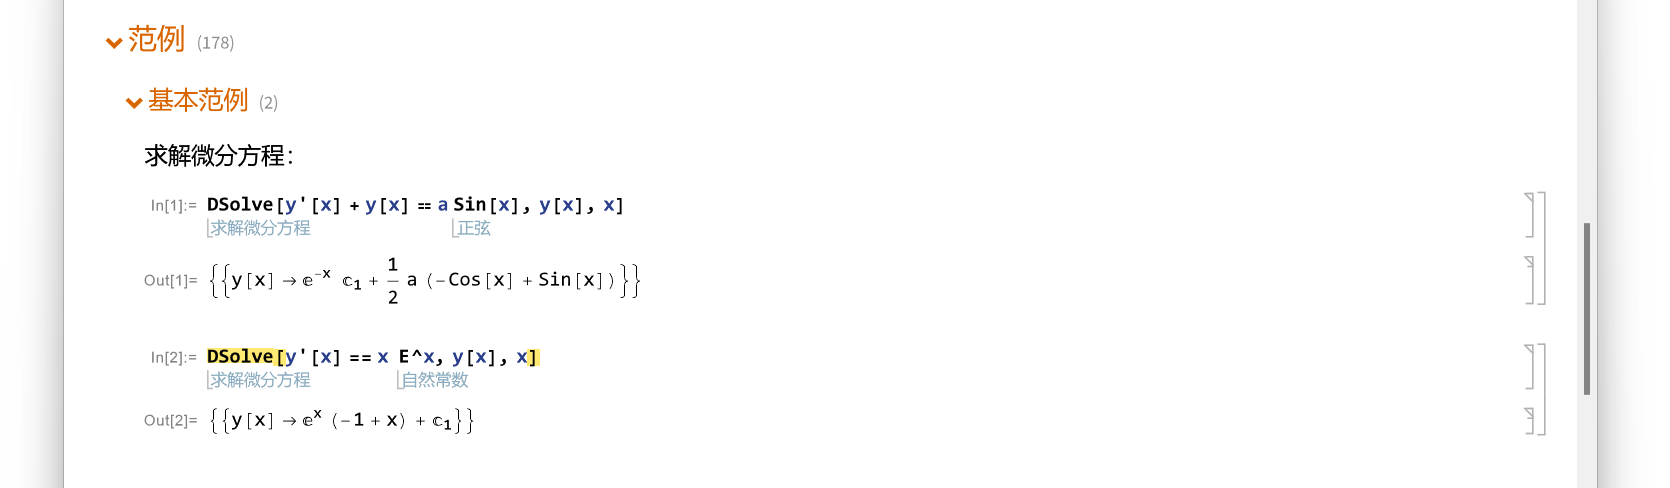
\includegraphics[width=.7\textwidth]{assets/software/MMA_edit_in_document.png}
  \caption{在 Mathematica 文档中编辑算例}
  \label{fig:MMA_edit_in_document}
\end{figure}

然而,尽管某些时候官方文档相当好用,但有时候软件厂商没有公开相关软件的文档,又或者官方文档写得相当晦涩难懂,再或者官方文档没有中文版本。这时,我们就需要寻找那些其他的民间教程了。

\section{善用互联网}

在\chapref{cha:how-to-find-solutions}中,我们已经介绍了如何在互联网上挑选内容,如「关注更新时间」「警惕洗稿文」等。那么,我们应该去哪儿寻找优质的网络教程呢?本节将推荐一些比较好的教程来源,并按推荐程度排序。

\subsection{各种「独立博客」}

在整个中文互联网上,有许许多多像我们一样的独立博客博主——所谓的「独立博客」,指的是有自己的网站(例如,《你缺计课》网页版的网址是 \url{https://www.criwits.top/missing},这个网址完全由我们自己控制,不隶属于任何一个其他的平台),只登载自己的文章的博客。经验上来说,这些独立博客的内容质量一般较高,因此我们将它们放在推荐的第一位。

比如,如果你想初步学习 \LaTeX{} 的使用,那么下面这篇文章就是一个非常不错的选择:

\begin{figure}[htb!]
  \centering
  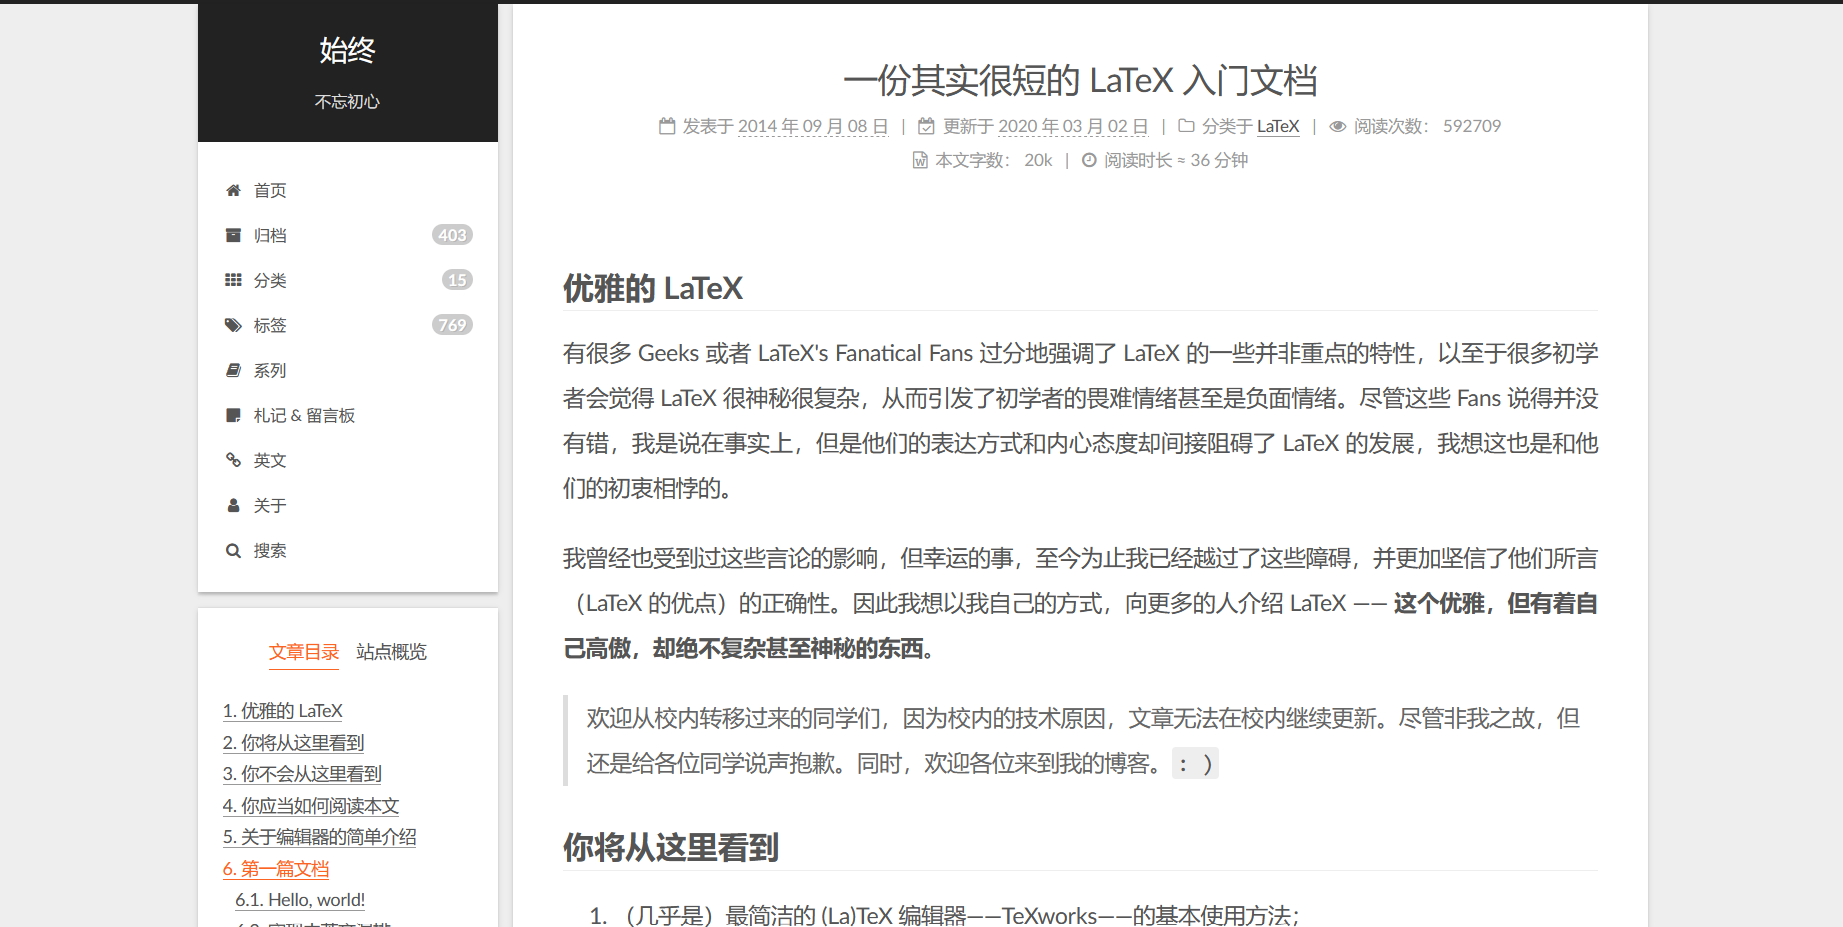
\includegraphics[width=.7\textwidth]{assets/software/LaTeX_tutorial.png}
  \caption{来自某独立博客的 \LaTeX{} 教程}
  \label{fig:LaTeX_tutorial}
\end{figure}

又比如,若你想学习编程,网上早已有博主为不同的编程语言编写了详细无比的入门教程:

\begin{figure}[htb!]
  \centering
  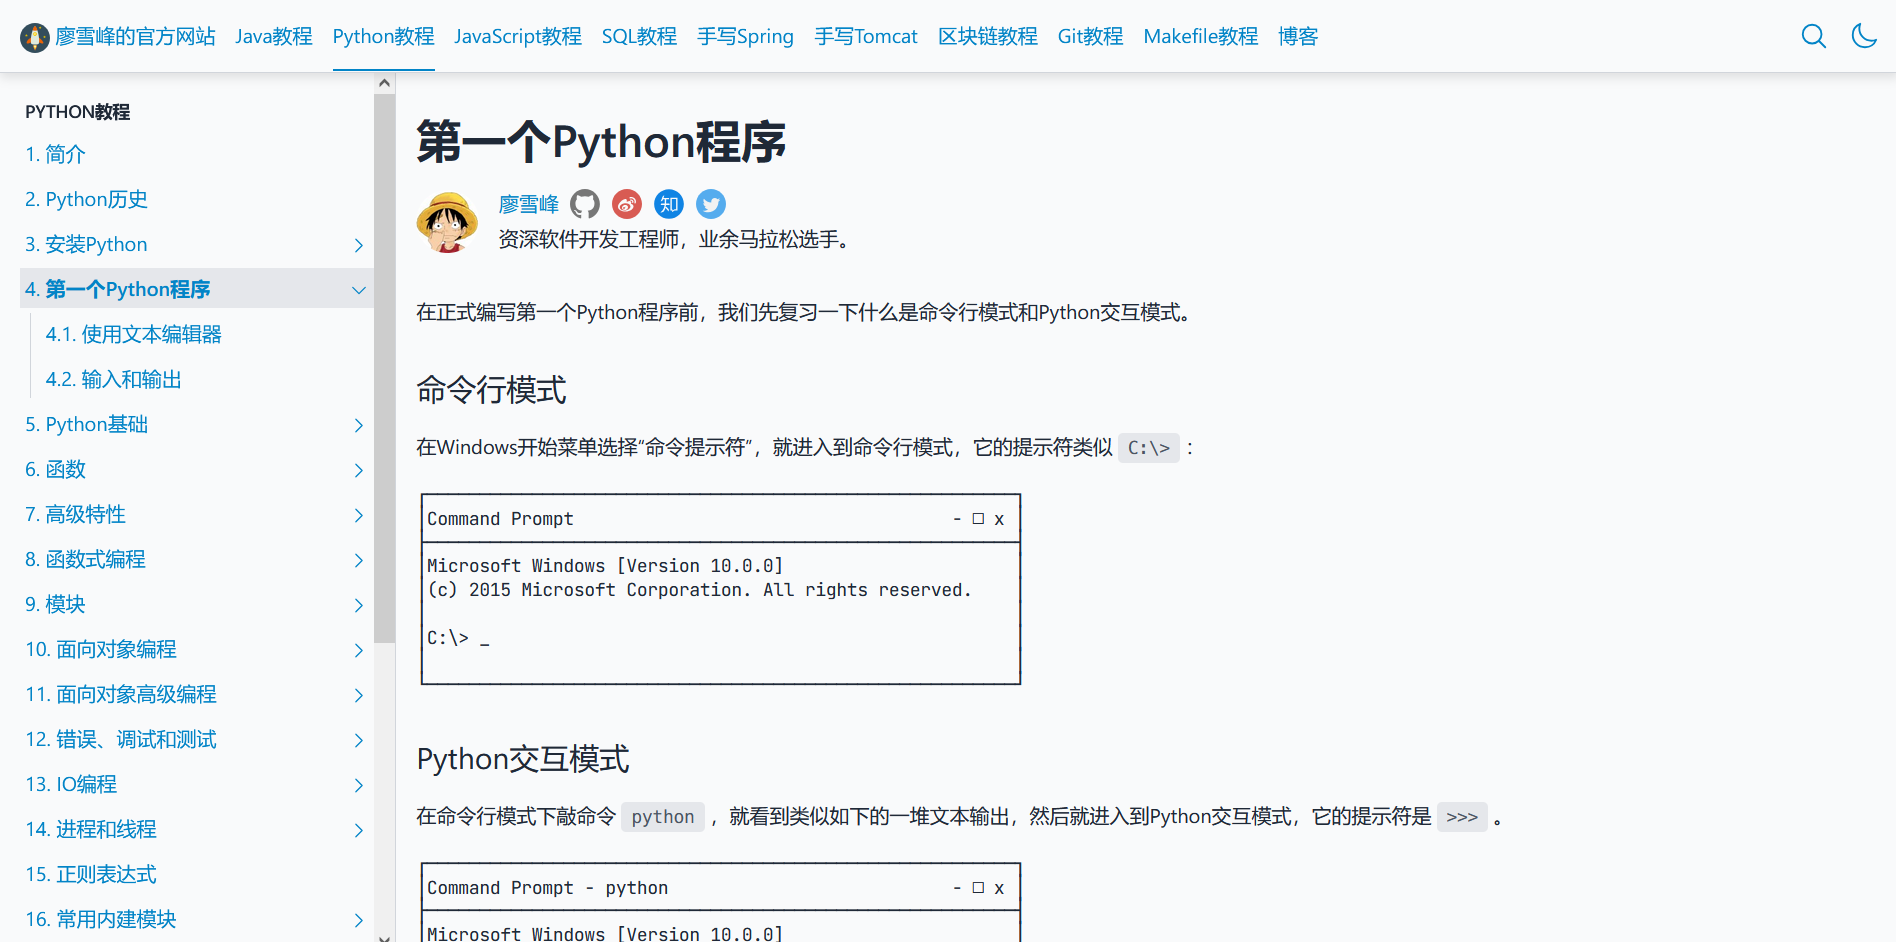
\includegraphics[width=.7\textwidth]{assets/software/LXF_mainpage.png}
  \caption{有多种编程语言的入门教程的独立博客}
  \label{fig:LXF_mainpage}
\end{figure}

但将独立博客上的文章作为教程,缺点也很明显:首先,这样的内容通常「可遇不可求」——毕竟,这些博客分散在互联网的各处,能不能发现「宝藏」,全靠运气。其次,这些文章的覆盖面终究有限。博主们大都不是专门做教程的人,因而不太可能讲解到我们所需要学习的每一款软件。

受限于我们的见识积累,我们显然无法为大家总结出一个「优质博客列表」。你可以在互联网上探索的过程中,不断地发现那些符合自己口味的博客和博主,并将它们分享给更多有需要的人。

\subsection{各种中文网络平台}

在诸如 CSDN、博客园、哔哩哔哩等常见中文网络平台上,充满了各种各样的软件使用教程,其中不乏优质的作品。在这些平台上,我们往往能找到一些教程供自己参考。例如,如果你想学习视频剪辑,那么视频网站上有大量的相关软件教程可以观看;你想学习文字排版,在相关论坛里必然有很多专业人士分享经验;至于学习各种开发类、技术类软件,那么一些技术性博客网站里的海量文章一定能满足你的需求。另一方面,在微信上,还有许多撰写或翻译各种优质软件教程的公众号,它们往往侧重于某一个领域(例如,软件开发或者建筑设计),时常推送相关软件的教程推文。

对于各种网络平台,我们可以直接在它们的搜索框中检索关键字,然后依据点击量或评论数等来轻松地筛选出更可能是优质内容的教程。比如,在视频网站上搜索「Revit 教程」,然后选择【最多播放】来将结果按播放量排序。

\begin{figure}[htb!]
  \centering
  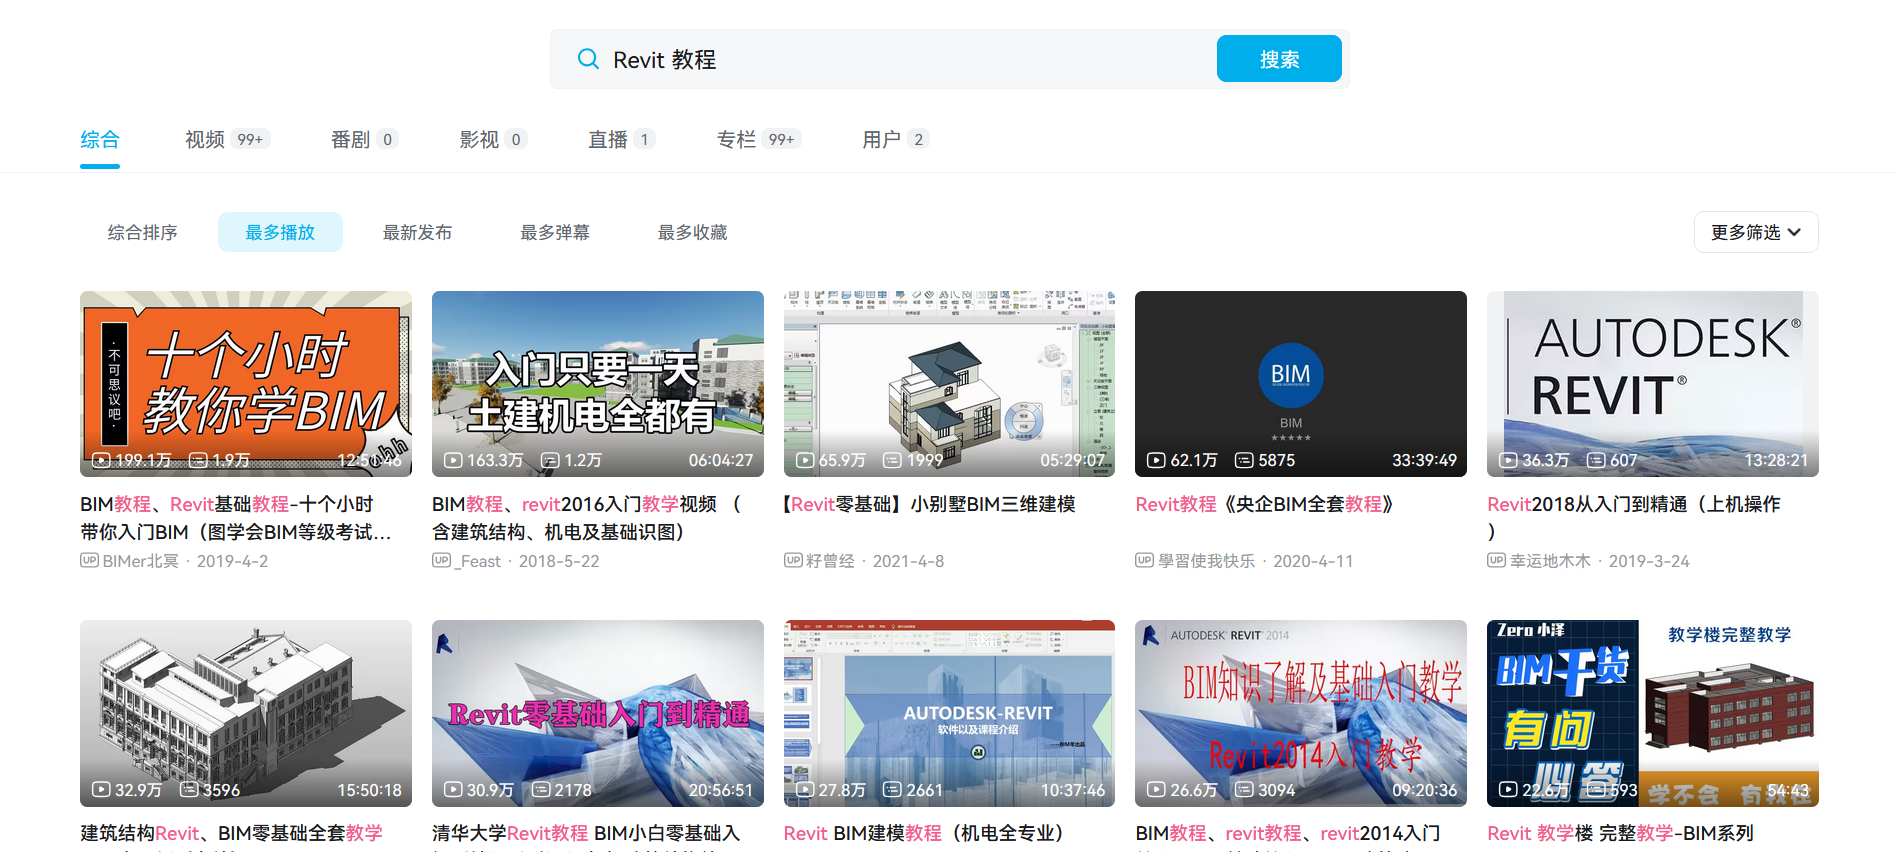
\includegraphics[width=.8\textwidth]{assets/software/Searching_Revit_tutorials_on_bilibili.png}
  \caption{搜索「Revit 教程」视频}
  \label{fig:Searching_Revit_tutorials_on_bilibili}
\end{figure}

而微信公众号——某种程度上它更像是低门槛的独立博客——则更多地依赖「口口相传」这样的方式来获得关注。如同我们在\chapref{cha:software-installation}中提到的那种「软件分享类公众号」一般,这里的「教程类公众号」也需要我们主动挖掘,你可以通过其他途径去了解感兴趣的领域中的优良公众号。

在之前的章节我们已经介绍过,目前网上普遍存在「洗稿」现象:一些人原文复制他人的文章——复制也就算了,还复制不全,抄来的东西都是错的。许多内容是 AI 生成的,内容胡编乱造,充满错误。此外,有些平台还存在「假标题」的现象,部分页面吸引人点击却没有任何实质内容。还有些平台会出现「机翻国外网站教程」的现象,翻译质量嘛……不如不翻译。因此,我们在查找教程时应当主动地有所侧重,并在选择教程时审慎行事。

\subsection{或许,你需要「英文教程」}

如果你的英语水平不错,那么当现有的中文资料无法满足你的需求时,不妨在必应等国际化的搜索引擎上,使用英语检索相应的资料。例如,如果你想系统入门「Ansys」这款结构仿真计算软件,但无论是各种中文博客上的文章,还是哔哩哔哩上的教学视频,都不合你口味,那么你可以试试搜索「Ansys Tutorial」。搜索结果中除了 Ansys 的官方教程之外,还有许多国外高校相应课程的讲义。你可以简要阅读来挑选符合自己喜好的内容。

\begin{figure}[htb!]
  \centering
  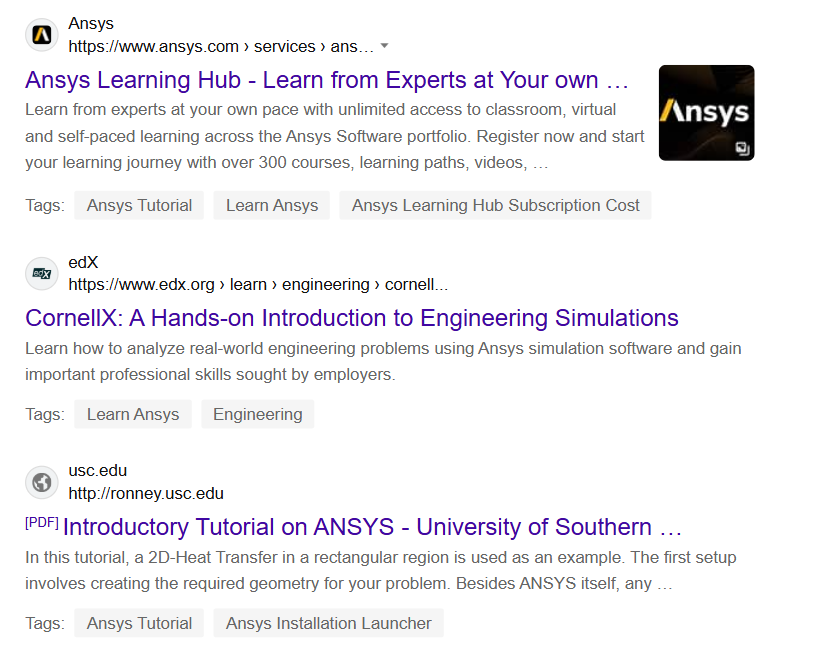
\includegraphics[width=.6\textwidth]{assets/software/Ansys.png}
  \caption{Ansys 英语教程}
  \label{fig:Ansys}
\end{figure}

当然,在浩如烟海的互联网上,英语内容也有精品和糟粕。在本章和\chapref{cha:how-to-find-solutions}中介绍的内容挑选方法,此时依然适用。而当你使用软件遇到教程未涉及的内容,或你有特定需求时,也可以按照之前我们介绍的方法寻找问题的解决方案。

\practice

\begin{enumerate}
  \item 试着在网上寻找一篇来自独立博客的,用于你常用软件的优质教程。
  \item 试着分别在中文和英文互联网平台上查找你最近正在学或即将学习的软件的教程。
\end{enumerate}
